\chapter{显微成像系统的检测实验}

通过搭建实验检测平台,对光学薄膜的表面缺陷通过进行观测检测验证。对照本 显微成像检测系统的原理框图搭建实验平台,通过显微成像实验平台,实验完成对照 明光源的位置设置、显微图像采集格式的设置、树莓派接口通信的调试,以及对图像 数据采集传输与控制进行测试,验证了光学薄膜表面缺陷检测系统具备可行性。

\section{薄膜表面缺陷检测测试}

\subsection{实验仪器介绍和安装}
该平台分为两部分安装,一部分为实验装置的安装,后对系统烧录后进行驱动安装和图像测试,测试成功后安装对应的Django框架和相应程序。

\subparagraph{硬件基础环境搭建}

首先组装实验装置平台,把设计的显微镜头和设计的 CMOS 驱动板通过 CS 口连 接起来,CMOS 驱动板的数据输出采用 FFC 软排线连接,组装好后的镜头如图 5.1 所示。
显微系统的照明光源采用环形白色 LED 的反射式照明,根据外界不同的环境光 照,可以调节照明 LED 灯的亮度,以适应不同透明度的薄膜的照明要求。采集不同 光照强度下的显微图像,选取具有最佳对比度的图像作为最终需要识别处理的图像。 

其次是树莓派系统的启动。首先通过 SD 卡将 Raspbian
系统写入树莓派中,插入 SD 卡后,系统会自动启动。
使用ssh客户端软件或者命令行通过路由连接树莓派,startx后进入
pi 的登录界面,输入账号和密码,Raspbian 的默认账号
和密码分别为 pi 和raspberry。

树莓派摄像头的配置及启动调试: 首先进行
摄像头的硬件设置,RPi 固件和 raspi-config 已为摄像
头更新,接着通过执行apt-get 系列升级和补丁命令来进行系统更新,然后重启树莓派即可。最
后通过相关摄像头命令sudo raspi -config 使pi 摄像
头的CSI接口生效,选择 Enable Camera 回车。摄像头使能后,在树莓派官网上根据需求下载相应camera驱动和二进制包进行测试。
\begin{figure}[h]
\centering
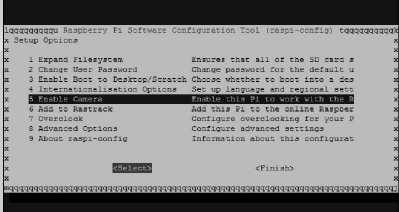
\includegraphics[width=0.7\linewidth]{Figure/rasp_4}
\caption{安装系统界面}
\label{fig:rasp_4}
\end{figure}

\subparagraph{软件系统设置(未完成)}
需要进行Django的安装和Server机的安装,


搭建的实验系统平台如图 所示,连接显微镜头和 CMOS 采集板,采用反射式 的照明方式,打开上位机软件界面,并调节好显微镜焦距,观测镜片表面的薄膜,如 图 所示。
%\subparagraph{使用方式解释说明}

\subsection{缺陷检测结果分析(未完成)}
在显微成像系统测试中,选取了实验室最常用的光学透镜的表面薄膜,观测了增 透膜和增反膜表面的缺陷程度,对表面出现的缺陷进行了分析。调整不同的光照方式, 对同一片增透膜进行了多次检测,以消除光照对检测误差的影响,通过采集不同的薄膜 显微图像,并对传输上来的图片进行了图像预处理,采用均值滤波算法滤除高斯噪声, 并对图像进行二值化处理,对采集的多幅图像进行比较选择,排除对焦不同等差异条 件。采集到的薄膜表面的显微图像原始数据。
在上位机上对显微图像采用中值滤波进行图像降噪预处理,处理 结果如图所示。
采用阈值分割处理算法对预处理过的图像做缺损检测处理,选定标准完整的薄膜 表面图像作为标准背景图,将显微系统采集到的带有缺损的薄膜表面图像与之对比, 对缺陷图像进行阈值分割处理,并截取放大显示识别出的典型的缺陷形状,选取记录 结果如下所示。

在对薄膜的缺陷检测实验中,CMOS 相机采集的速度在 1080P 格式下可以达到每秒 30 帧,通过 CSI 接口传到显示器,实现了对薄膜的实时检测和识别,还能够通过网口传 到局域网实现远程缺陷检测。相比传统的缺陷检测系统,整个缺陷检测系统硬件上采 用了性价比的 ARM 处理器,选用手机上常用的 CMOS 图像传感器 IMX135,并通过 CSI-2 串 行接口输出图像,实现了高速实时的检测特点。整个检测系统结构紧凑,Raspbian 操 作系统可更新升级,实现了微型化智能化的检测特点。
\subsection{本章小节}
本章搭建了基于树莓派处理器的显微成像系统平台,选用不同光照强度的光源进 行照明,测试了实验室的光学薄膜表面的缺陷,验证了该系统的实时检测性能,并对 采集的薄膜表面的图像进行处理,识别出缺陷的类型和形状,达到了系统的总体设计要求。
